%% ID: newtoni
%% QUESTIONS: firing_the_rockets
%% CONCEPTS: newtonii, newtoniii, vectors, calculus
%% LEVEL: 2
%% TOPIC: mechanics/dynamics
%% TYPE: physics
%% TITLE: Newton's First Law
%% ORDER: 12

% This is the template that sets out all of the Problems and produces the Exercise/Solution labels and numbering
% There are two classes of Exercise: "problem" which has a Question and Solution, and "hint" which has a Question, Hint and Solution

% This is the template that sets out all of the Problems and produces the Exercise/Solution labels and numbering
% There are two classes of Exercise: "problem" which has a Question and Solution, and "hint" which has a Question, Hint and Solution

% These are the packages to use in all documents, and the paper size to use:
\documentclass[a4paper,11pt]{article}
\usepackage[usenames,dvipsnames]{xcolor}
\usepackage[margin=1.5cm]{geometry}
\usepackage{amsmath}
\usepackage{amssymb}
\usepackage{color}
\usepackage{graphicx}
\usepackage{graphics}
\usepackage[margin=1.5cm]{geometry}
\usepackage{fancyhdr}
\usepackage{float}
\usepackage{lscape}
\usepackage[font={small},labelfont=bf]{caption}
\usepackage{ifthen}
\usepackage{enumitem}
\usepackage{subcaption}		%Allows grouped figures. The percentage sign after the first \end{subfigure} puts them side by side, omitting it puts one above the other.
\usepackage{graphicx,xcolor} 	%Allows the use of colour in the files
\usepackage{centernot} 		%Puts the / in a not equal to sign in the centre, use as \cnot{...}
\usepackage{comment} 		%Allows \begin{comment} .... \end{comment} to comment out bulk text.
\usepackage{etoolbox}		%Allows the boolean flags and the \toggletrue and \togglefalse commands
\usepackage{cancel}		%Allows the crossing out of terms in maths mode to show they cancel out
\usepackage{wrapfig}

%Packages for font choices
\usepackage{palatino}
\usepackage{mathpazo}


%Then where to find the graphics:
%WARNING -  relative to the TeX file being compiled - NOT this template!
		\graphicspath{{../Diagrams/}{Diagrams/}{./}} %This allows diagrams: {{As a sister folder to Latex}{A subdirectory of LaTeX}{Or just in LaTeX itself}}

% WARNING -  If you want the diagrams to be a sister folder to the LaTeX folder - pdflatex.exe sometimes needs an extra argument to cope with the "../" part; usually it can only cope with subdirectories as opposed to parent ones. If it refuses to compile and says it cannot find the diagrams, either add "--shell-escape" to the start of the arguments of pdflatex, OR move the diagrams to a subdirectory of the one containing the TeX files.
%In TeXworks, to add the extra argument, go to Edit -> Preferences -> Typesetting -> Processing Tools. Click on "pdfLaTeX" -> Edit -> "+" button, then type "--shell-escape" (without quotes) and press the up arrow twice so that it becomes top of the list.


%Then any custom commands written, along with shortcuts and variables:
% This document contains any custom commands, shortcuts and variables needed for the files to compile. It is called by "Problem_Template.tex" and so needs to be in the same directory.

%Defines vectors universally, for ease of editing and consistency.
\newcommand{\vtr}[1] {\mathit{\underline{\boldsymbol{#1}}}}

%Draws a big red box containing the text as in \ALERT{<TEXT HERE>}. For labelling draft copies with important notes.
\def\ALERT#1{\begin{center}\colorbox{red}{\hbox{\textcolor{black}{\textbf{#1}}}}\end{center}}

%Roman-style subscript; removes math-mode font.
\def\s#1{_\textrm{#1} }

%The operators in integrals and derivatives.
\def\d{\operatorname{d}\!}

%The Euler e should be in Roman font.
\def\e{\textrm{e}}

%The Rutherford title, to save typing and for consistency:
\def\Rutherford{Rutherford School Physics}
\def\Concepttitle#1{\noindent\textsc{\Rutherford\vspace{0.4cm}\\ \LARGE Physical Concept: \textbf{#1}}}
\def\Problemtitle#1{\noindent\textsc{\Rutherford\vspace{0.4cm}\\ \LARGE Website Problems: \textbf{#1}}}
\def\AddProblemtitle#1{\noindent\textsc{\Large \Rutherford ~ --- ~ Additional Problems\vspace{0.4cm}\\ \LARGE \textbf{#1}}}
%\def\AddProblemtitle#1{\noindent\textsc{\Rutherford\vspace{0.4cm}\\ \LARGE Additional Problems: \textbf{#1}}}

%define quick question to be used in eg concept sheet.
%\def\qq#2{#1}{\color{red}[#2]\color{black}}
\newcommand{\qq}[2]{\nl Quick Question:\hspace{1 mm} #1\color{red}\hspace{2 mm} Answer:\color{black}\hspace{1 mm}  #2}
\newcommand{\stress}[1]{\emph{#1}}

%%%%%%%%%%%   some definitions used in latexing the CQMP:
% fractions that are of right size in set equations
\def\half{{\textstyle \frac{1}{2}}}
\def\quarter{{\textstyle \frac{1}{4}}}
\def\third{{\textstyle \frac{1}{3}}}
\def\eighth{{\textstyle \frac{1}{8}}}

% obtain a new line
\def\nl{\hfil\break}
\def\nll{\\ \\ \noindent}



%creates numbered lists with a), then i.
\renewcommand{\theenumi}{\alph{enumi}}% first level are latin characters
\renewcommand{\labelenumi}{\theenumi)} %tells it to put a bracket after the character.
\renewcommand{\theenumii}{\roman{enumii}}%second level are little roman characters
\renewcommand{\labelenumii}{\theenumii.} %tells it to put a dot after the character
 % In a file called "Definitions.tex" in the same directory as this file.

%Define some boolean switches:
\newtoggle{solutions_only}	%Print only the solutions
\newtoggle{no_solutions}		%Don't print any solutions  (overridden by solutions_only)
\newtoggle{solutions_at_end}	%Print the solutions at end (overridden by solutions_only and no_solutions)
\newtoggle{no_credits}		%Don't print the credit arguments

%Use this to write a list of things needed to know for a section. It automatically won't print when "solutions_only" is on.
%Its only argument should be a list of things needed to know in "\item [....]" form
\newenvironment{knowledge}[1]{
\iftoggle{solutions_only}{}{It is assumed that students will be familiar with the following concepts:
\begin{itemize} #1 \end{itemize}
\vspace{0.5cm}}
}

%Allows the headings to be managed when not printing problems ect.
\newenvironment{Qsection}[1]{
%\iftoggle{solutions_only}{}{\section{#1}} %Don't output headings in the solutions(?)
\iftoggle{solutions_at_end}{\AtEndDocument{\section{#1}}}{}
\section{#1}
}

\newenvironment{Qsubsection}[1]{
%\iftoggle{solutions_only}{}{\subsection{#1}} %Don't output headings in the solutions(?)
\iftoggle{solutions_at_end}{\AtEndDocument{\subsection{#1}}}{}
\subsection{#1}
}

%Set the values of the boolean switches: Yes - "toggletrue", No - "togglefalse".
\togglefalse{solutions_only}	%	ONLY		Output only solutions? 
\togglefalse{no_solutions}		%	NONE		Don't output solutions at all? 
\togglefalse{solutions_at_end}	%	END		Output solutions at the end?
\togglefalse{no_credits}		%			Don't output the credit field
%All 8 cases have been tested; ONLY takes precedence, then NONE and finally END is lowest.


%##############################################################################################################
%											Then the bulk of the layout options:
%##############################################################################################################

\setlength{\topmargin}{-2cm}
%\setlength{\oddsidemargin}{0.5cm}
%\setlength{\evensidemargin}{0.5cm}


%##############################################################################################################


\newcounter{exercisenumber}%[chapter] %counter is set to zero when "chapter" appears
\def\theexercisenumber{\arabic{exercisenumber}}


\iftoggle{no_solutions}{}{ %Put a header at the end before the solutions, and reset the counter. Only if solutions are being printed AND at the end.
	\iftoggle{solutions_only}{}{
		\iftoggle{solutions_at_end}
			{\AtEndDocument{\newpage \part*{Solutions:} \setcounter{exercisenumber}{0} \setcounter{section}{0}}}{}
	}
}


%%%%%%%%%%%%%%%%%%%%%%%%%%%%%%%%%%%%%%%%%%%%%%%%%%%%%%%%%%%%%%%%%%%%%%%%%%%%%%%%%
%Creates \begin{problem}[label]{exercise_text}{source_text}{solution_text}\end{problem} command - the label argument is optional
%If put in, remember to put in [] brackets.  A label called label.ex will be generated.
\newenvironment{problem}[4][noref]{
 \refstepcounter{exercisenumber} %\refstepcounter allows you to reference to the exercise number
%
\iftoggle{solutions_only}{\hfil\break \textit{Solution}~\theexercisenumber:  #4}{ %If only solutions, just output solution.
	\noindent{\textit{Exercise}~\theexercisenumber:}
	\ifthenelse{\equal{#1}{noref}}{}{\label{#1.ex}} #2 %\vspace{0.3cm}
	\iftoggle{no_credits}{}{
			%\hfil\break {\small #3} \vspace{0.3cm} %This is the old line, replaced with the one below, without the ifthenelse statement; in case something goes wrong.
			\ifthenelse{\equal{#3}{}}{}{ {\tiny [#3]} \vspace{0.3cm}} %If the credit field is blank; don't bother printing it or the space for it.
	} %reference argument
%
	\iftoggle{no_solutions}{}{ %If the solutions aren't to be printed, do nothing.
		\iftoggle{solutions_at_end}
			{\AtEndDocument{\stepcounter{exercisenumber}\hfil\break \textit{Solution}~\theexercisenumber:  #4 \vspace{0.5cm}}} %If at the end: do this.
			{\hfil\break \textit{Solution}~\theexercisenumber:  #4} 	%Else leave in line as in TeX file.
	}
}

\vspace{0.2cm}}

%%%%%%%%%%%%%%%%%%%%%%%%%%%%%%%%%%%%%%%%%%%%%%%%%%%%%%%%%%%%%%%%%%%%%%%%%%%%%%%%%
%Creates \begin{hint}[label]{exercise_text}{hint_text}{source_text}{solution_text}\end{hint} command - the label argument is optional
%If put in, remember to put in [] brackets.  A label called label.ex will be generated.
\newenvironment{hint}[5][noref]{
 \refstepcounter{exercisenumber}
%
\iftoggle{solutions_only}{\hfil\break \textit{Solution}~\theexercisenumber:  #5}{  %If only solutions, just output solution.
	\noindent{\textit{Exercise}~\theexercisenumber:}
	\ifthenelse{\equal{#1}{noref}}{}{\label{#1.ex}} #2 \vspace{0.1cm}
	 \hfil\break  \textit{Hint:}  #3{} %\vspace{0.3cm}
	\iftoggle{no_credits}{}{
			\ifthenelse{\equal{#4}{}}{}{\\ \hfil {\tiny #4} \vspace{0.3cm}} %This is the old line, replaced with the one below, without the ifthenelse statement; in case something goes wrong.
			%\ifthenelse{\equal{#4}{}}{}{{\tiny [#4]} \vspace{0.3cm}} %If the credit field is blank; don't bother printing it or the space for it.
	} %reference argument
%
	\iftoggle{no_solutions}{}{%If the solutions aren't to be printed, do nothing.
		\iftoggle{solutions_at_end}
			{\AtEndDocument{\stepcounter{exercisenumber}\hfil\break \textit{Solution}~\theexercisenumber:  #5 \vspace{0.5cm}}} %If at the end: do this.
			{\hfil\break \textit{Solution}~\theexercisenumber:  #5}%Else leave in line as in teX file.
	}
}
\vspace{0.2cm}}

%%%%%%%%%%%%%%%%%%%%%%%%%%%%%%%%%%%%%%%%%%%%%%%%%%%%%%%%%%%%%%%%%%%%%%%%%%%%%%%%%


 %%%%%%%
\newenvironment{additional}[2][noref]{
 \refstepcounter{exercisenumber}
% \vspace{.2cm}
\nl
\noindent{\textit{Exercise}~\theexercisenumber:}
\ifthenelse{\equal{#1}{noref}}{}{\label{#1.ex}} #2 }{%\vspace{5.1cm}
 }
%










% to mark as a draft.  Comment both these lines out when complete.  The page number will return to the footer.
%\pagestyle{myheadings}
%\markright{\textcolor{red}{\textbf{DRAFT: \today}}}


\begin{document}
\addtolength{\topmargin}{0.0 cm}
\setlength{\columnsep}{22pt}
\Concepttitle{Newton's First Law of Motion}

\section{As Newton stated it...}

Every body continues in its state of being at rest or in uniform motion unless acted upon by a resultant force.
\setlength{\columnsep}{22pt}
\section{Application of Newton I}
\subsection*{Levels 1-3}
\begin{wrapfigure}{r}{6cm}
\vspace{-2.0cm}
\center
\includegraphics[width=0.3\textwidth]{../../figures/FreeBody1.eps}
\caption{The free body diagram of the forces acting {\it on a cardboard box} at rest on a table, where $W$= weight of the box and $N$ is the normal reaction of the table on the box.  The forces on the table are not drawn here.}\vspace{-3.5cm}
\end{wrapfigure}

There are two things that we should note in relation to this law:
\begin{enumerate}
\item Often we forget the important second part of this law - that it applies to bodies that are moving at constant velocity, not just those that are at rest.   

\item When we look at bodies in equilibrium - where all the forces are balanced and there is no acceleration - we often think that we are applying Newton's Second Law but actually it is Newton's First Law that tells us there must be zero\\
resultant force.

\end{enumerate}
{\bf For example}, a cardboard box is {\it at rest} on a table, what is the magnitude of the normal reaction of the table on the box? \\

\noindent We begin with the free body force diagram for the box.  Newton's First Law tells us that, as the box is in equilibrium (at rest), the sum of all the forces must equal zero (technically all the torques must also be equal to zero but we will come on to that at a later level).
\begin{eqnarray}
N-W=0 \\
N=W
\end{eqnarray}
Therefore the normal reaction {\it of the table on the box} is equal to the weight of the box.

\subsection*{Quick Questions}
[Where appropriate take the acceleration due to gravity to be, $g=10$ ms$^{-2}$.]
\qq{A box is being dragged along a frictional floor by a tension, $T=10$ N, in a rope that is parallel to the ground.  If the box is moving at constant velocity what is the magnitude of the frictional force that must be acting on the box?}
{$F=10$ N}
\qq{A wooden block of mass, $10$ kg, rests on a frictional plane that is inclined at an angle of $30^\circ$ to the horizontal.  What is the magnitude and direction of normal reaction of the plane on the block if the block remains at rest?}
{Normal reaction $=10g\cos(30^\circ)=50\sqrt{3}$ N, direction is perpendicular to the plane}
\qq{A trailer of mass , $M$, containing 10 blocks, each of mass $m$, is at rest on a frictional plane that is inclined at an angle of $\theta$ to the vertical.  What is the magnitude and direction of the normal reaction of the plane on the trailer?}
{Normal reaction $=(M+10m)g\sin(\theta)$, direction is perpendicular to the plane}


\subsection*{Levels 4+}
\setlength{\columnsep}{22pt}
\begin{wrapfigure}{r}{6cm}
\center
\includegraphics[width=0.3\textwidth]{../../figures/FreeBody2.eps}
\caption{The free body diagram of the forces acting {\it on a cardboard box} that is moving at a constant velocity, $v$, parallel to the surface of a frictional table, where $W$= weight of the box, $N$ is the normal reaction of the table on the box, $F$ is the frictional force applied to the box by the table and $P$ is the pulling force we need to apply to keep the box at constant velocity, $v$. } \label{NI2}\vspace{15.0cm}
\end{wrapfigure}
Newton's First Law applies in 1, 2 or 3 dimensions and we can apply it in any direction.  If a body is at rest or continuing at constant velocity then the resultant force in any direction must be equal to zero.  Let us imagine a box that is being dragged along parallel to the surface of a {\it frictional} table at a constant velocity, $v$, as shown in figure \ref{NI2}. What can we work out about the normal reaction, $N$, and the force, $P$, that we need to apply to the box in order to maintain this constant velocity?\\
Newton's First Law tells us that the sum of all forces must equal zero both parallel and perpendicular to the table's surface, therefore
\begin{eqnarray}
N-W&=&0 \ \ \mbox{therefore} \ \ N=W \ \ \mbox{and}\\
P-F&=&0 \ \ \mbox{therefore}\ \  P=F
\end{eqnarray}
\subsection*{Quite Quick Questions}
[Where appropriate take the acceleration due to gravity to be, $g=10$ ms$^{-2}$.]

\qq{A box is being dragged along the floor by the tension, $T=10$ N, in a rope, where the rope is inclined at an angle of $30^o$ to the ground.  If the box is moving at constant velocity what is the magnitude of the frictional force that must be acting on the box?  What is the magnitude of the normal reaction of the ground on the box if the mass of the box is $1$ kg?}\\
{$F=T\cos(30)=5\sqrt{3}$ N; \nl
$N+T\sin(30)-mg=0$\ therefore\nl
$N=mg-T\sin(30)=10-5 = 5$ N}
\qq{A wooden block of mass, $10$ kg, rests on a frictionless, inclined plane at angle of $30^\circ$ to the horizontal and is held in place by a rope running parallel to the surface of the plane.  What is the magnitude and direction of normal reaction of the plane on the block? What is the tension in the rope?} \\
{$N=10g\cos(30)=50\sqrt{3}$ N, direction is perpendicular to the plane;\nl $T=10g\sin(30)=5g=50$ N.}
\qq{A trailer of mass, $M$, containing 10 blocks, each of mass $m$, moves at constant velocity up a frictionless, inclined plane via a rope that is, parallel to the surface of the plane, and attached to a motor.  The plane is angled at $\theta$ to the vertical.  What is the magnitude and direction of the normal reaction of the plane on the trailer? What is the tension in the rope?}\\
{$N=(M+10m)g\sin(\theta)$, direction is perpendicular to the plane; \nl $T=(M+10m)g\cos(\theta)$.}




\end{document}
